
\documentclass[12pt]{article}
%\pagenumbering{arabic} 

\usepackage[margin=1in]{geometry}
\usepackage{fancyhdr}
\pagestyle{fancy}
\usepackage{algorithm,algpseudocode}
\usepackage{amsmath}
\usepackage{amssymb}
\usepackage{amsmath}
\usepackage{amsfonts}
\usepackage{amssymb}
\usepackage{amsthm}
\usepackage{graphicx}
\usepackage[affil-it]{authblk}
\usepackage{setspace}
\usepackage{bm}
\usepackage[round]{natbib}
\usepackage{booktabs,multirow}
\usepackage{titlesec}
\usepackage{algorithm,algpseudocode}
\usepackage[subrefformat=parens]{subfig}
%\usepackage{subcaption}
\usepackage{csvsimple}
\usepackage{siunitx}
\usepackage[figuresright]{rotating}
\usepackage{tikz,pgfplots}
\pgfplotsset{compat=newest}
%\usepackage{natbib}
\usepackage{apalike}
\usepackage{tabularx} 
\usepackage{siunitx}
\usepackage{etoolbox}
\pagenumbering{arabic}
\newcommand{\diff}{\mathop{}\!d}
\DeclareMathOperator*{\argmin}{arg\,min}
\usetikzlibrary{arrows,calc,decorations.pathreplacing,shapes.geometric,topaths,shapes.misc,shapes.multipart,patterns}
\usepackage{algorithm,algpseudocode}% http://ctan.org/pkg/{algorithms,algorithmx}

\algnewcommand{\Set}[1]{%
	\State \textbf{Set:}
	\Statex \hspace*{\algorithmicindent}\parbox[t]{.8\linewidth}{\raggedright #1}
}
\algnewcommand{\Initialize}[1]{%
	\State \textbf{Initialize:}
	\Statex \hspace*{\algorithmicindent}\parbox[t]{.8\linewidth}{\raggedright #1}
}

\usepgfplotslibrary{groupplots}
\usepgfplotslibrary{statistics}
\algnewcommand{\algorithmicgoto}{\textbf{go to}}%
\algnewcommand{\Goto}[1]{\algorithmicgoto~\ref{#1}}%


\usepackage[colorinlistoftodos,prependcaption,textsize=tiny]{todonotes}

\usepackage{graphicx}
\usepackage{lscape}
\usepackage{kotex}
%\usepackage{romannum}
\newtheorem{thm}{Theorem}
\newtheorem{cor}{Corollary}
\newtheorem{exa}{Example}
\newtheorem{ass}{Assumption}
\newtheorem{pro}{Proposition}
\newtheorem{defn}{Definitions}
\newtheorem{lem}{Lemma}
\newtheorem{pf}{proof}
\newtheorem{remark}{Remark}
\newtheorem{ex}{Exercise}
\newcommand*{\comb}[1][-1mu]{\permcomb[#1]{C}}
\lhead{Column Generation Techniques for GAP}
\rhead{김예린 연구노트}
%\rhead{}

\begin{document}
	\title{Column Generation Techniques for GAP}
	\author{}
	\date{\today}
	\maketitle
	
\section{Preliminary Tests}
Github page : \texttt{https://github.com/mody3062/CG}
\paragraph{Testing algorithms}
\begin{itemize}
	\item Classical column generation (Kelly's cutting plane)
	\item Stabilized column generation (O. Du Merle, et. al., 1997)
	\item Separation + Classical column generation
	\item Separation + Stabilized column generation
\end{itemize}


\paragraph{Algorithmic parameters}

RMP was constructed with a single decision variable which is dummy. The coefficient of the dummy variable on the objective function was set to a sufficiently large value, which is the sum of listed values such that \verb|np.sum(c,axis=1)|. For stabilized column generation algorithm, I changed the parameter $\epsilon$ from 0.01 to 0.0001 for every 100 trials. (I am not sure whether I could understand the criteria for changing the parameter value($\epsilon$) well.)


 To start the column generation procedure, an initial re-
stricted master problem has to be provided. This initial
restricted master problem must have a feasible LP relax-
ation to ensure that proper dual information is passed to
the pricing problem. We have chosen to start with one
column for each agent, corresponding to the optimal knap-
sack solution, and a dummy column consisting of all ones
with a large negative profit. The dummy column ensures
that a feasible solution to the LP relaxation exists. This
dummy column will be kept at all nodes of the branch-and-
bound tree for the same reason.


\begin{landscape}
	\begin{table}[]
		\resizebox{1.3\textwidth}{!}{%
			\begin{tabular}{lllllllllllllllll}
				\hline 
				&  & \multicolumn{3}{c}{Kelly} &  & \multicolumn{3}{c}{Stab.} &  & \multicolumn{3}{c}{Sep.} &  & \multicolumn{3}{c}{Sep.+Stab.} \\ \cline{3-5} \cline{7-9} \cline{11-13} \cline{15-17} 
				&  & iteration & total(s) & M(\%) &  & iteration & total(s) & M(\%) &  & iteration & total(s) & M(\%) &  & iteration & total(s) & M(\%) \\			\hline \\[-3mm]
				d05100 &  & 2485 & 26.13 & 25\% &  & 2216 & 33.27 & 32\% &  & 2296 & 44.57 & 61\% &  & 2321 & 49.8 & 66\% \\
				d10100 &  & 1223 & 7.83 & 25\% &  & 1068 & 11.49 & 42\% &  & 949 & 6.38 & 32\% &  & 858 & 7.25 & 40\% \\
				d10200 &  & 4485 & 133.04 & 54\% &  & 4423 & 199.37 & 61\% &  & 3253 & 132.49 & 67\% &  & 3703 & 193.21 & 73\% \\
				d20100 &  & 852 & 3.67 & 26\% &  & 782 & 6.63 & 49\% &  & 673 & 3.24 & 29\% &  & 629 & 4.15 & 41\% \\
				d20200 &  & 2513 & 38.59 & 41\% &  & 2549 & 65.75 & 55\% &  & 1862 & 32.86 & 51\% &  & 2288 & 52.38 & 59\% \\
				e05100 &  & 2577 & 15.03 & 42\% &  & 2356 & 27.73 & 51\% &  & 3487 & 74.37 & 86\% &  & 2761 & 37.61 & 76\% \\
				e10100 &  & 1345 & 6.83 & 36\% &  & 1405 & 12.45 & 52\% &  & 1160 & 6.64 & 54\% &  & 1261 & 8.93 & 58\% \\
				e10200 &  & 6273 & 153.91 & 77\% &  & 6580 & 271.2 & 80\% &  & 4328 & 186.97 & 87\% &  & 4455 & 218.22 & 88\% \\
				e20100 &  & 942 & 3.13 & 32\% &  & 979 & 7.4 & 52\% &  & 711 & 2.81 & 36\% &  & 644 & 3.5 & 46\% \\
				e20200 &  & 3273 & 37.77 & 57\% &  & 3374 & 76.73 & 69\% &  & 2390 & 44.17 & 75\% &  & 2713 & 61.78 & 78\%\\ \hline
			\end{tabular}%
		}
	\end{table}
\end{landscape}


\begin{figure}[] 
	\begin{center}
		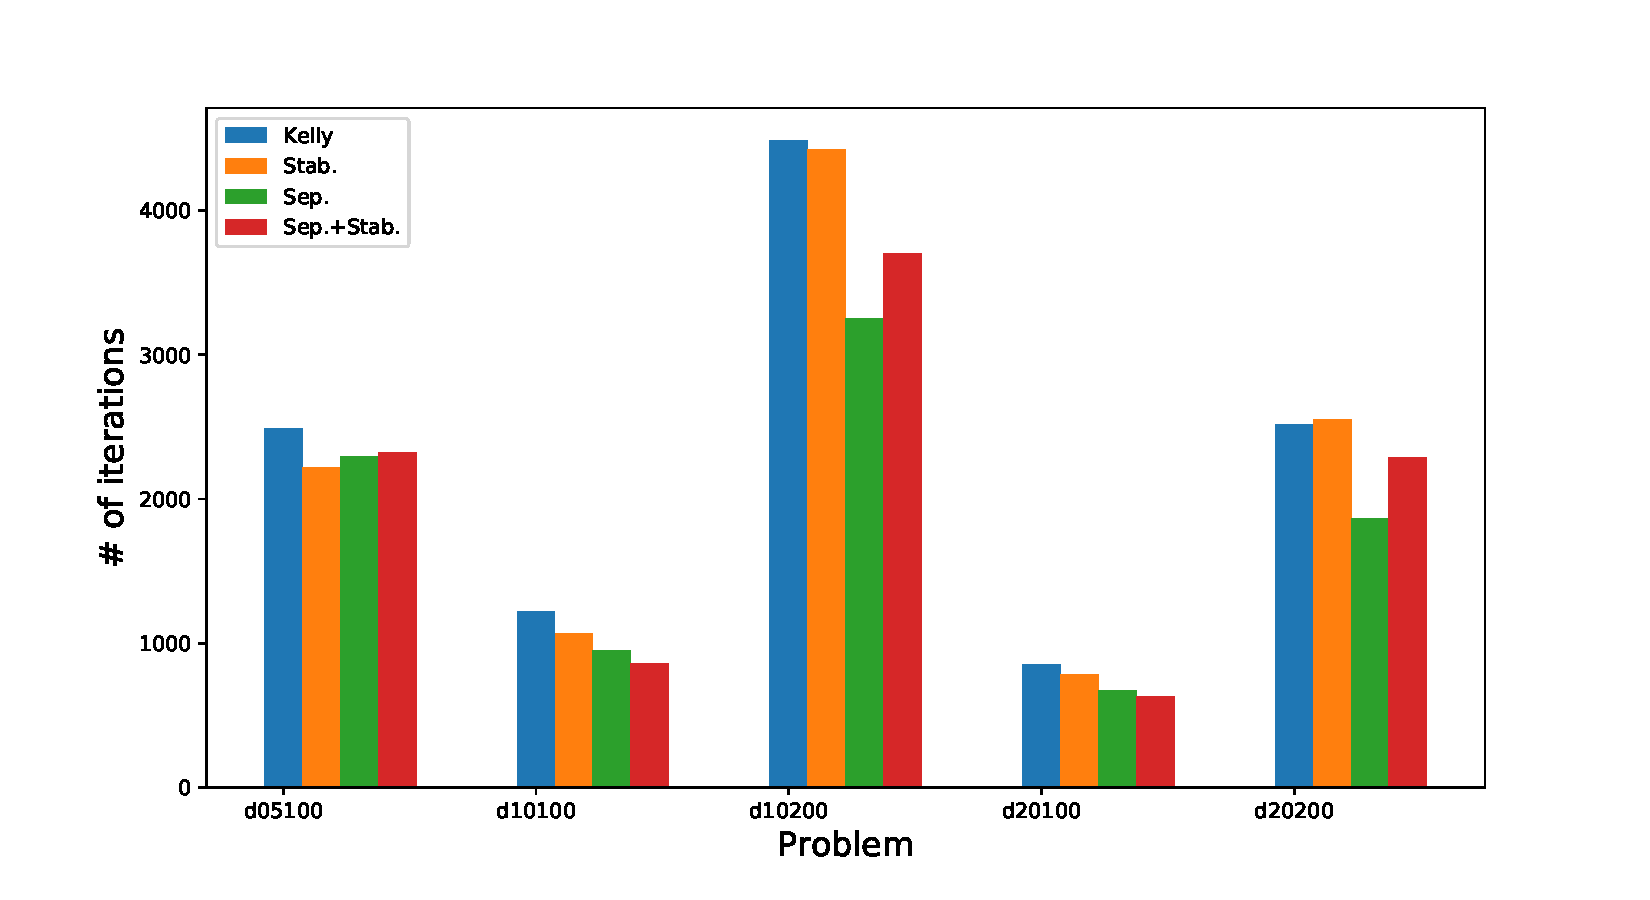
\includegraphics[width=0.8\textwidth]{d}
\caption{ Performance comparison of the algorithms (gap\_d)}
	\end{center}
\end{figure}


\begin{figure}[] 
	\begin{center}
		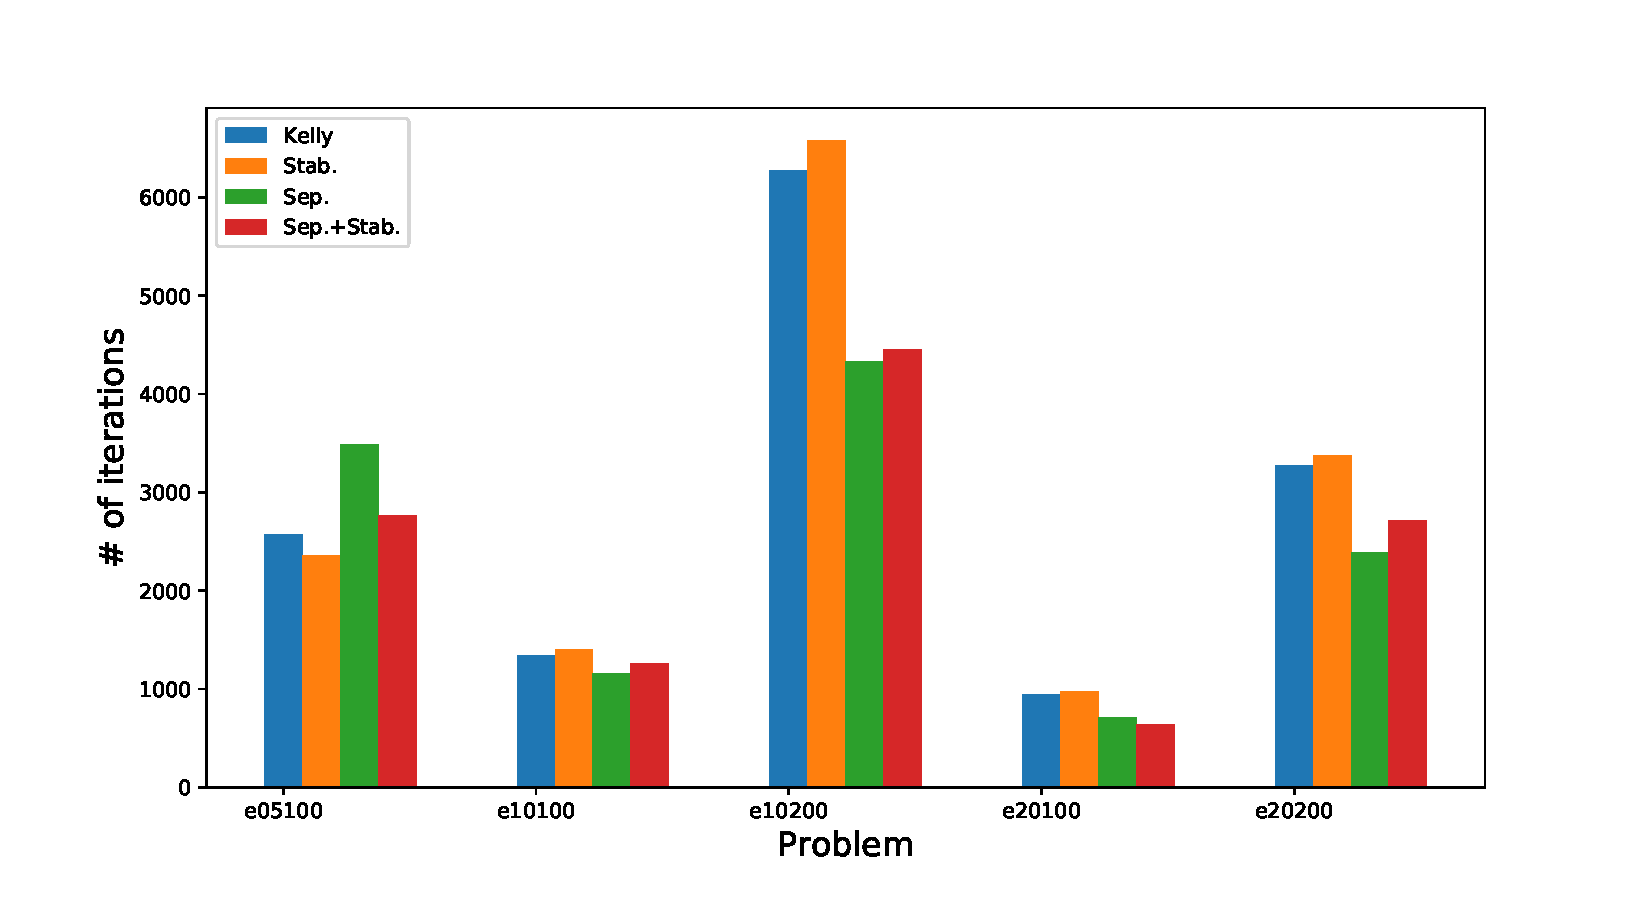
\includegraphics[width=0.8\textwidth]{e}
		\caption{ Performance comparison of the algorithms (gap\_e)}
	\end{center}
\end{figure}
\end{document}